\chapter{Faster models}
\label{chapter:fastermodels}

Models presented in chapter \ref{chapter:testingandcomparing} are quite slow,
giving us only $\sim$ 3-4 frames per second on NVIDIA Jetson TX2. 
In this chapter we experiment with light-weight variations of ResNet and SegNet. We also test
various mobile models proposed in recent years capable of running on devices with
low computational power. From now on, we use only Deggendorf dataset, binary crossentropy loss
and images in RGB color space.

\section{Reducing the number of parameters}
\label{sec:reduce_params}

As stated above, our models (namely ResNet and SegNet) are slow in terms of inference time.
The first idea that comes to our mind is to reduce the number of parameters in order
to get more FPS.\\

Our \textbf{ResNet} contains so called \textit{identity blocks} which we put in
pairs next to each other. The model also takes parameter \textit{f} which denotes the
filter multiplier (default 16) being used in all layers.
\textbf{SegNet} contains too many layers so we decided to reduce them and experiment
with the number of filters in each convolutional layer.

List of modified models:

\begin{itemize}
    \item ResNet-1 - original model, $f=8$
    \item ResNet-2 - original model, $f=4$
    \item ResNet-3 - every other identity block skipped, $f=16$
    \item ResNet-4 - every other identity block skipped, $f=8$
    
    \item SegNet-1 - filters by layers: 64, 128, 256, 256, 256, 256, 128, 64, 32
    \item SegNet-2 - filters by layers: 32, 64, 128, 128, 256, 128, 128, 64, 32
    \item SegNet-3 - filters by layers: 32, 32, 64, 64, 128, 128, 64, 32, 32
    \item SegNet-4 - filters by layers: 32, 32, 64, 64, 64, 64, 64, 32, 32
\end{itemize}

\begin{table}[h]
	\centering
	\begin{tabular}{|c||c|c|c|c|c|c|c}
	    \hline
		model & \# params & on Jetson & train acc & train IoU & test acc & test IoU\\
		\hline
		ResNet-1 & 698,017 & 0.13288 sec & 0.9795 & 0.9509 & 0.9408 & 0.8836 \\
		\hline
		ResNet-2 & 179,297 & 0.10143 sec & 0.9678 & 0.9332 & 0.9360 & 0.8796 \\
		\hline
		ResNet-3 & 1,895,649 & 0.16817 sec & 0.9783 & 0.9488 & 0.9446 & \textbf{0.8919} \\
		\hline
		ResNet-4 & 480,817 & \textbf{0.09807 sec} & 0.9662 & 0.9284 & 0.9399 & 0.8850 \\
		\hline
		\hline
		SegNet-1 & 2,534,401 & 0.31107 sec & 0.9444 & 0.9024 & 0.9316 & 0.8784 \\
		\hline
		SegNet-2 & 1,075,009 & 0.22216 sec & 0.9497 & 0.9073 & 0.9365 & 0.8816 \\
		\hline
		SegNet-3 & 391,105 & 0.14389 sec & 0.9631 & 0.9276 & 0.9417 & \textbf{0.8889} \\
		\hline
		SegNet-4 & 206,145 & \textbf{0.13818} sec & 0.9625 & 0.9268 & 0.9380 & 0.8843\\
		\hline
	\end{tabular}
	\caption[Results of modified ResNet and SegNet training]{Results of modified ResNet and SegNet training.}
	\label{tab:reduced_resnet_segnet}
\end{table}

\begin{figure}[!h]
	\centerline{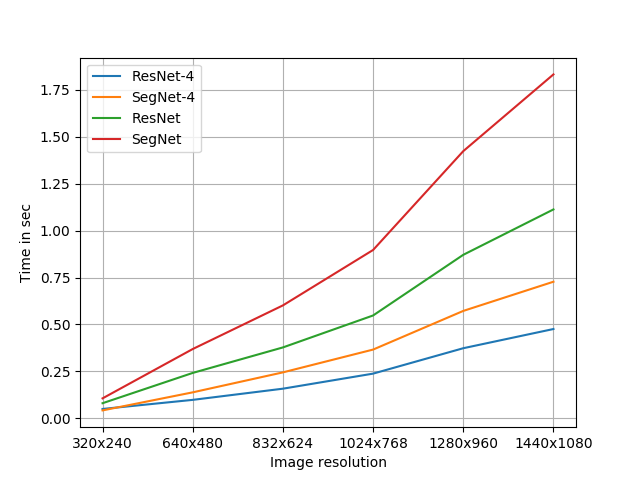
\includegraphics[width=0.9\textwidth]{images/inference_times.png}}
	\caption[Comparison of inference times against various image resolutions]{Comparison of inference times against various image resolutions on Jetson TX2 GPU.}
	\label{img:inference_times_comparison}
\end{figure}

By reducing ResNet's number of parameters we are able to increase the FPS to 10
while preserving the IoU. The same applies to SegNet where we reach 7 FPS
with the same IoU, see Table \ref{tab:reduced_resnet_segnet}.

We have also tried incorporating dilation rate to
encoder convolutional layers \cite{bib:yu2015multi}. In case of SegNet, we set
the dilation factors in ascending order (1, 2, 4, 8). ResNet contains identity
and bottleneck blocks, both of them having one $3\times 3$ convolutional layer. We 
tried setting dilation rate just in identity block. Other experiments with ResNet
involved setting dilation rate in both identity and bottleneck blocks.
The experiments show that dilation convolutions do not bring improvement in terms of
accuracy to our models.

Aforementioned models are able to process images of various resolutions. Figure
\ref{img:inference_times_comparison} shows the comparison of inference times of
these models against several resolutions (with aspect ratio 4:3). Predictions
of images with resolution $320\times 240$ take similar amount of time. However, with
growing resolution we can see modified ResNet beats other models and is a good choice
when dealing with higher resolutions.


\section{Mobile models}
\label{sec:mobile_models}

\begin{table}[h]
	\centering
	\begin{tabular}{|c||c|c|c|c|}
	    \hline
		name & encoder & decoder & $\alpha$ & \# params \\
		\hline
        SSeg-1 & ShuffleNet ($g=1$) & SkipNet 8s & 0.25 & 970,825 \\
        SSeg-2 & ShuffleNet ($g=1$) & SkipNet 8s & 0.5 & 1,920,793 \\
        SSeg-3 & ShuffleNet ($g=2$) & SkipNet 8s & 0.25 & 959,241 \\
        SSeg-4 & ShuffleNet ($g=2$) & SkipNet 8s & 0.5 & 1,889,841 \\
        SSeg-5 & ShuffleNet ($g=4$) & SkipNet 8s & 0.25 & 921,833 \\
		\hline
		SNetV2-1 & ShuffleNetV2 & DeepLabV3+ & 1.0 & 1,871,428 \\
		SNetV2-2 & ShuffleNetV2 & DeepLabV3+ & 0.5 & 694,886 \\
		\hline
		MNetV2-1 & MobileNetV2 & DeepLabV3+ & 1.0 & 11,978,698 \\
		MNetV2-2 & MobileNetV2 & DeepLabV3+ & 0.5 & 4,643,466 \\
		MNetV2-3 & MobileNetV2 & DeepLabV3+ & 0.25 & 2,742,418 \\
		MNetV2-4 & MobileNetV2* & DeepLabV3+ & 0.25 & 1,252,498 \\
		\hline
		MNetV3-L-1 & MobileNetV3-Large & DeepLabV3+ & 1.0 & 4,641,674 \\
		MNetV3-L-2 & MobileNetV3-Large & DeepLabV3+ & 0.5 & 2,484,146 \\
		MNetV3-L-3 & MobileNetV3-Large & DeepLabV3+ & 0.25 & 1,902,602 \\
		\hline
		MNetV3-S-1 & MobileNetV3-Small & DeepLabV3+ & 1.0 & 2,142,074 \\
		MNetV3-S-2 & MobileNetV3-Small & DeepLabV3+ & 0.75 & 1,775,474 \\
		\hline
	\end{tabular}
	\caption[Description of mobile models]{Description of mobile models we experiment with.
	$\alpha$ denotes width multiplier. MNetV2-4 contains encoder MobileNetV2 where we removed
	final convolution layer to reduce the number of parameters.}
	\label{tab:mobilenets_desc}
\end{table}

Mobile models are quite popular when it comes to real-time performance on devices
with low computation resources. Since our robot lacks real-time prediction ability,
we decided to search for a modern mobile model, that would allow the robot to deal
with this problem. Based on previous works in this field, we test \textit{ShuffleSeg}
\cite{bib:gamal2018shuffleseg}, \textit{ShuffleNetV2} \cite{bib:turkmen2019efficient},
\textit{MobileNetV2} \cite{bib:sandler2018mobilenetv2} and both large and small versions
of \textit{MobileNetV3} \cite{bib:howard2019searching}. Although authors of MobileNetV2 and
MobileNetV3 use other decoders in their original articles, we decided to use DeepLabV3+ 
\cite{bib:chen2018encoder} in our experiments. In fact, we were not able to reproduce
learning ability of \textit{Lite R-ASPP} as a decoder proposed for MobileNetV3 and
DeepLabV3+ seems like a good fit for our purposes. In Table \ref{tab:mobilenets_desc}
we present architecture and hyper-parameters of mobile models. All model variations are 
trained using \textit{Adam} optimizer and the training procedure took from 25 to 40 minutes in
all cases.

\begin{table}[h]
	\centering
	\begin{tabular}{|c||c|c|c|c|c|}
	    \hline
		name & train acc & train iou & test acc & test iou & on Jetson \\
		\hline
        SSeg-1 & 0.8776 & 0.8849 & 0.8862 & 0.8548 & 0.05559 sec \\
        SSeg-2 & 0.8112 & 0.9141 & 0.8096 & 0.8565 & 0.07858 sec \\
        SSeg-3 & 0.8442 & 0.8919 & 0.7391 & 0.8618 & 0.07048 sec \\
        SSeg-4 & 0.7327 & 0.9166 & 0.7676 & 0.8581 & 0.08932 sec \\
        SSeg-5 & 0.8013 & 0.9144 & 0.8060 & 0.8343 & 0.08605 sec \\
		\hline
		SNetV2-1 & 0.9811 & 0.9547 & 0.9506 & 0.8979 & 0.08615 sec \\
		SNetV2-2 & 0.9731 & 0.9386 & 0.9375 & 0.8799 & 0.06318 sec \\
		\hline
		MNetV2-1 & 0.9757 & 0.9457 & 0.9433 & 0.8852 & 0.24385 sec \\
		MNetV2-2 & 0.9760 & 0.9441 & 0.9424 & 0.8849 & 0.14537 sec \\
		MNetV2-3 & 0.9746 & 0.9411 & 0.9341 & 0.8721 & 0.09902 sec \\
		MNetV2-4 & 0.9757 & 0.9453 & 0.9396 & 0.8770 & 0.08698 sec \\
		\hline
		MNetV3-L-1 & 0.9711 & 0.9369 & 0.9486 & 0.8918 & 0.13953 sec \\
		MNetV3-L-2 & 0.9744 & 0.9440 & 0.9549 & \textbf{0.9000} & 0.10666 sec \\
		MNetV3-L-3 & 0.9734 & 0.9417 & 0.9485 & 0.8908 & 0.07009 sec \\
		\hline
		MNetV3-S-1 & 0.9733 & 0.9418 & 0.9506 & 0.8933 & 0.06125 sec \\
		MNetV3-S-2 & 0.9739 & 0.9430 & 0.9536 & 0.8977 & \textbf{0.05534} sec \\
		\hline
	\end{tabular}
	\caption[Results of mobile models training]{Results of mobile models trained on Deggendorf dataset along with their inference times measured on Jetson TX2.}
	\label{tab:mobilenets_results}
\end{table}

Results of trained models are summarized in Table \ref{tab:mobilenets_results}. ShuffleSeg's
all modifications are quite fast, but their test IoUs are much lower compared to other models. 
SNetV2-1 gives us promising results with $11.5$ FPS. All versions of MobileNetV2 do not reach
test IoU higher than $89\%$ and are not that fast as expected. With decreasing $\alpha$ the
IoU decreases as well. MobileNetV3 seems to be most efficient one. Although its large version's
test IoU is the best compared to all mobile models tested, the inference time is too high.
A good trade-off between IoU and inference time provides MNetV3-L-3 with $14.2$ FPS. But
surprisingly, both small versions of MobileNetV3 beat other models with their significantly better
performance. We are able to get to 18 FPS with unchanged IoU.

We picked one variation of each model which gives us the best trade-off between IoU and speed
and compared them with our small models using AUC-ROC curve. The graph presented in Figure
\ref{img:mobilemodels_roc} shows that all MobileNets are the most powerful ones while
ShuffleNet being equal with our modified ResNet and SegNet. 

\begin{figure}[!h]
	\centerline{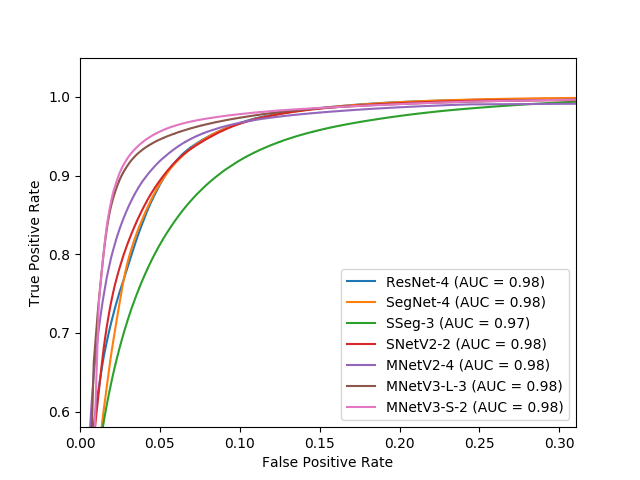
\includegraphics[width=0.9\textwidth]{images/mobilemodels_roc.png}}
	\caption[Comparison of mobile models using AUC-ROC curve]{Comparison of mobile models using AUC-ROC curve. The graph is zoomed to the upper-left corner for better view.}
	\label{img:mobilemodels_roc}
\end{figure}